\documentclass[11pt]{article}
\usepackage[margin=1in]{geometry}\usepackage{amsmath,amssymb,amsthm,booktabs,graphicx,hyperref}
\newtheorem{lemma}{Lemma}\newtheorem{definition}{Definition}
\title{Support-Controlled Harmonic Reversal Asymmetry and Exact Inversion-Quotient Allocation in Bach Chorales and WJazzD}
\author{Anonymous}\date{Draft, September 2026}
\begin{document}\maketitle
\begin{abstract}
We measure how far harmonic progressions are from time-reversible, at the level of chord-to-chord transitions quotiented by transposition, in two public symbolic corpora: 430 Bach chorales (music21 corpus, 26249 chord changes, 67 key-relative states) and 412 Weimar Jazz Database solos (27491 chord changes, 175 states, grouped into 273 compositions). The estimand is the held-out log-ratio of forward to reversed transition counts, $\sigma$, scored on work-grouped folds. Bilaterally observed edges carry 0.765 to 0.832 bits per transition in Bach and 1.555 to 2.670 in WJazzD (retained-total and conditional estimands), so the asymmetry is not an artifact of one-way transitions. A KL chain-rule lemma gives an exact allocation $\sigma_{C_{12}}=\sigma_{D_{12}}+\Delta_{\mathrm{inv}}$ between inversion-invariant and inversion-resolving components, closing to machine precision on every event. In Bach, inversion orientation carries 0.137 to 0.156 bits per transition, 16.0 to 16.2\% of the reversal score, with chorale-level 95\% lower bounds of 0.128 to 0.145; in WJazzD it carries 3.7 to 4.7\% with composition-level lower bounds of 0.053 to 0.089, positive but below our preregistered 0.10-bit threshold. Cycle affinities and a spanning-forest circulation basis localise the asymmetry in cadential and turnaround loops. We cite Gonz\'alez-Espinoza, Mart\'inez-Mekler and Lacasa (2020) as the direct predecessor on melodic time irreversibility and claim no theorem novelty for the quotient identity.
\end{abstract}

\part*{I. Logic}
\section{Prior musical irreversibility and claim boundary}
Time irreversibility of music has been quantified before: Gonz\'alez-Espinoza, Mart\'inez-Mekler and Lacasa (2020) applied horizontal-visibility-graph statistics to scalar melodic note streams across 8{,}856 pieces. We quantify a different object, the reversal asymmetry of transposition-quotiented harmonic transition laws, and localise it through inversion-sensitive, directed-edge and closed-cycle analyses. The quotient identity we use is a corollary of the KL chain rule and of exact coarse-graining results (Esposito, 2012; Teza and Stella, 2020); it is stated as a lemma because it fixes the estimand and prevents an incorrect quotient implementation, not as a contribution.

\section{Harmonic edge laws, reversal and bilateral-support estimands}
\begin{definition}A chord event is a key-relative 12-bit pitch-class mask with mode (the annotated tonic at pitch class 0); consecutive identical masks are collapsed to chord changes (an uncollapsed control is reported). A directed edge is a pair $(i,j)$ of consecutive states; $R(i,j)=(j,i)$ is reversal. For an edge law $\mu$, $\sigma(\mu)=D_{\mathrm{KL},2}(\mu\Vert R_*\mu)$ in bits.\end{definition}
Held-out scoring: for work-grouped folds, each held-out edge receives $d_{ij}=\log_2\frac{c_{ij}+\alpha}{c_{ji}+\alpha}$ from training counts; the event mean estimates $\sigma$. Bilateral support restricts to edges with $c_{ij},c_{ji}\ge r$ in training; the retained-total estimand assigns excluded edges zero, the conditional estimand averages over retained edges only.

\section{Diagonal $C_{12}$ quotient and the chain-rule lemma}
\begin{lemma}[quotient identity; standard]Let $G=\mathbb Z_{12}$ act diagonally on edges, $T_g(i,j)=(gi,gj)$, and let reversal commute with the action. For the symmetrised law $\mu^G=\frac{1}{12}\sum_g (T_g)_*\mu$ and the orbit map $q$, $\sigma(\mu^G)=\sigma(q_*\mu)$.\end{lemma}
Proof: KL chain rule for the statistic $q$; both symmetrised laws are uniform within each orbit, so the conditional term vanishes. Our key-relative representation is the tonic-anchored orbit representative (an exact unsmoothed check on the common support gives identity gap $0.0$ in Bach; smoothed plug-ins differ because pseudocounts must be pushed forward, not added per cell).

\section{Exact $C_{12}\rightarrow D_{12}$ allocation}
Let $\kappa$ be mode-conditioned pitch-class inversion ($p\mapsto -p$) and $h$ the further quotient identifying an edge with its inversion. Since $h$ commutes with reversal, the chain rule gives, exactly and per event,
\[\sigma_{C_{12}}=\sigma_{D_{12}}+\Delta_{\mathrm{inv}},\qquad \Delta_{\mathrm{inv}}=\sum_z (h_*P)(z)\,D\big(P(\cdot\mid z)\Vert Q(\cdot\mid z)\big)\ge0,\]
with $P$ the $C_{12}$ law, $Q=R_*P$, and $h_*P$ obtained only by pushforward. $\Delta_{\mathrm{inv}}$ is the part of reversal asymmetry that requires distinguishing an interval structure from its inversion. The mode covariate is held fixed under $\kappa$; this is one valid $D_{12}$ action, not the unique music-theoretic one.

\section{Detailed balance, cycle affinities and circulation}
For a stationary first-order chain with flow $F_{ij}=\pi_iP_{ij}$, $\sigma=\sum_{i<j}(F_{ij}-F_{ji})\log_2(F_{ij}/F_{ji})$, and $\sigma=0$ iff detailed balance iff every cycle affinity $A_C=\sum_{(i,j)\in C}\log_2(F_{ij}/F_{ji})$ vanishes (Kolmogorov, 1936). With a spanning forest, $\sigma=\sum_C j_C A_C$ over fundamental cycles; individual terms are basis dependent, the total is not. A loop's affinity is a force, not a contribution: it is reported together with its circulation and with contiguous path counts.

\part*{II. Experiment}
\section{Corpora, states and grouped folds}
Bach: 430 chorales, 26249 collapsed chord changes, 67 states; folds by chorale. WJazzD: 412 solos in 273 compositions, 27491 collapsed chord changes, 175 states; folds by composition so performances of one tune never cross folds. Chord types are triads (Bach, music21 quality) and thirteen jazz symbol templates (WJazzD). State alphabets differ (67 versus 175), so raw magnitudes are not compared across corpora.

\section{Support-controlled held-out irreversibility}
\begin{table}[t]\centering\small\caption{Held-out reversal asymmetry by bilateral support (bits per transition). rho = share of held-out events on edges observed in both directions in training; retained-total assigns excluded edges zero; LCB = work- (Bach) or composition- (WJazzD) level 95\% lower bound.}\label{tab:sup}
\begin{tabular}{lrrrrrr}\toprule $\alpha$ & support & $\rho$ (\%) & retained-total & conditional & LCB & works with no retained edge \\ \midrule
\multicolumn{7}{l}{\emph{Bach chorales}} \\
0.1 & all & 100.0 & 0.966 & 0.966 & 0.975 & 0 \\
0.1 & r=1 & 95.9 & 0.798 & 0.832 & 0.809 & 0 \\
0.1 & r=2 & 93.9 & 0.741 & 0.789 & 0.747 & 0 \\
0.1 & r=5 & 89.1 & 0.617 & 0.692 & 0.618 & 0 \\
0.5 & all & 100.0 & 0.894 & 0.894 & 0.904 & 0 \\
0.5 & r=1 & 95.9 & 0.782 & 0.815 & 0.792 & 0 \\
0.5 & r=2 & 93.9 & 0.730 & 0.778 & 0.736 & 0 \\
0.5 & r=5 & 89.1 & 0.611 & 0.686 & 0.613 & 0 \\
1 & all & 100.0 & 0.855 & 0.855 & 0.865 & 0 \\
1 & r=1 & 95.9 & 0.765 & 0.798 & 0.775 & 0 \\
1 & r=2 & 93.9 & 0.718 & 0.765 & 0.724 & 0 \\
1 & r=5 & 89.1 & 0.605 & 0.678 & 0.606 & 0 \\
\multicolumn{7}{l}{\emph{WJazzD}} \\
0.1 & all & 100.0 & 3.209 & 3.209 & 2.700 & 0 \\
0.1 & r=1 & 60.9 & 1.625 & 2.670 & 1.411 & 14 \\
0.1 & r=2 & 56.3 & 1.486 & 2.641 & 1.297 & 17 \\
0.1 & r=5 & 46.5 & 1.137 & 2.445 & 0.962 & 20 \\
0.5 & all & 100.0 & 2.715 & 2.715 & 2.304 & 0 \\
0.5 & r=1 & 60.9 & 1.591 & 2.614 & 1.382 & 14 \\
0.5 & r=2 & 56.3 & 1.463 & 2.600 & 1.276 & 17 \\
0.5 & r=5 & 46.5 & 1.129 & 2.426 & 0.954 & 20 \\
1 & all & 100.0 & 2.490 & 2.490 & 2.120 & 0 \\
1 & r=1 & 60.9 & 1.555 & 2.555 & 1.350 & 14 \\
1 & r=2 & 56.3 & 1.438 & 2.556 & 1.254 & 17 \\
1 & r=5 & 46.5 & 1.118 & 2.404 & 0.945 & 20 \\
\bottomrule\end{tabular}\end{table}
Endpoint (piece boundary) marginals contribute 0.2\% (Bach) and 0.0\% (WJazzD) of the plug-in $\sigma$; merging states with fewer than five occurrences changes nothing. Figure~2 shows the support curves.
\begin{figure}[t]\centering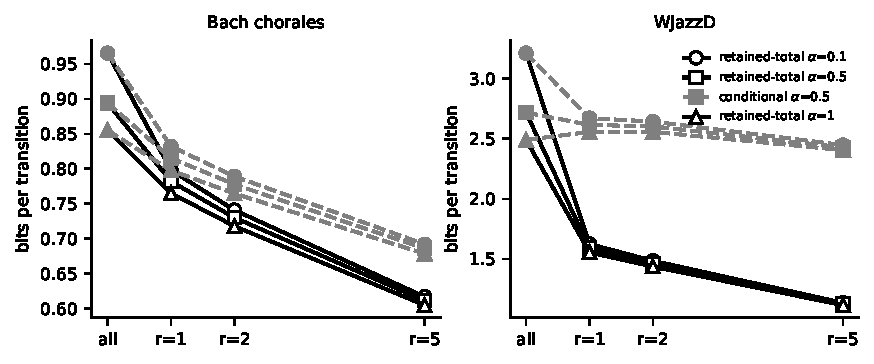
\includegraphics[width=\linewidth]{figs/fig2_support.pdf}\caption{Bilateral-support control: retained-total (solid) and conditional (dashed) scores across support thresholds and smoothing.}\end{figure}

\section{Inversion allocation and group inference}
\begin{table}[t]\centering\small\caption{Exact held-out $C_{12}\rightarrow D_{12}$ allocation (bits per transition). Per-event closure error $\le 9\times10^{-16}$. Group = chorale (Bach) or composition (WJazzD).}\label{tab:inv}
\begin{tabular}{llrrrrrr}\toprule corpus & $\alpha$ & $\sigma_{C}$ & $\sigma_{D}$ & $\Delta_{\mathrm{inv}}$ & share (\%) & group mean & group LCB \\ \midrule
Bach & 0.1 & 0.966 & 0.809 & 0.156 & 16.2 & 0.166 & 0.145 \\
Bach & 0.5 & 0.894 & 0.752 & 0.143 & 16.0 & 0.152 & 0.133 \\
Bach & 1 & 0.855 & 0.719 & 0.137 & 16.0 & 0.146 & 0.128 \\
WJazzD & 0.1 & 3.209 & 3.058 & 0.151 & 4.7 & 0.120 & 0.089 \\
WJazzD & 0.5 & 2.715 & 2.607 & 0.108 & 4.0 & 0.085 & 0.063 \\
WJazzD & 1 & 2.490 & 2.399 & 0.091 & 3.7 & 0.071 & 0.053 \\
Bach (uncollapsed) & 0.5 & 0.667 & 0.561 & 0.106 & 16.0 & 0.117 & 0.102 \\
WJazzD (uncollapsed) & 0.5 & 2.694 & 2.587 & 0.108 & 4.0 & 0.084 & 0.063 \\
\bottomrule\end{tabular}\end{table}
The preregistered conjunctive rule (group LCB $>0.10$ bits in both corpora at every $\alpha$) fails: the minimum is $0.053$ (WJazzD, $\alpha=1$). Bach passes at every $\alpha$ and its share is stable at 16.0 to 16.2\% across collapsed and uncollapsed events; WJazzD's share is 3.7 to 4.7\%. The absolute residuals are similar at $\alpha=0.1$ (0.137 versus 0.151 bits); the share contrast reflects WJazzD's three-fold larger inversion-invariant asymmetry. Standardising the two corpora to common weights over inversion-closed chord-family strata changes the share contrast from $0.120$ to $0.083$ ($E=0.30$).
\begin{figure}[t]\centering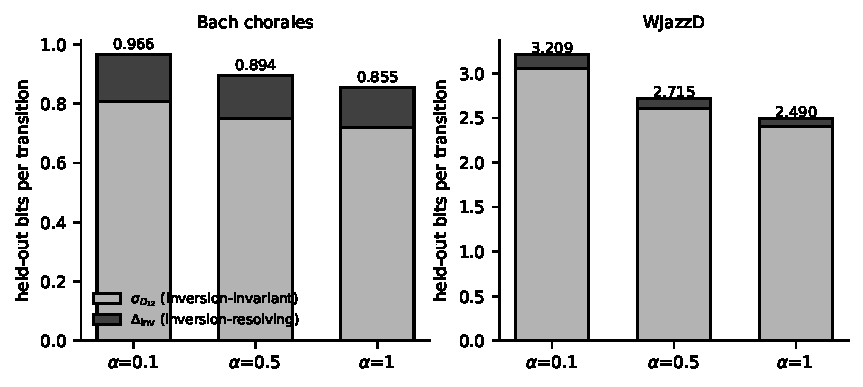
\includegraphics[width=\linewidth]{figs/fig3_decomposition.pdf}\caption{Exact allocation of held-out reversal asymmetry into inversion-invariant and inversion-resolving parts.}\end{figure}
\begin{figure}[t]\centering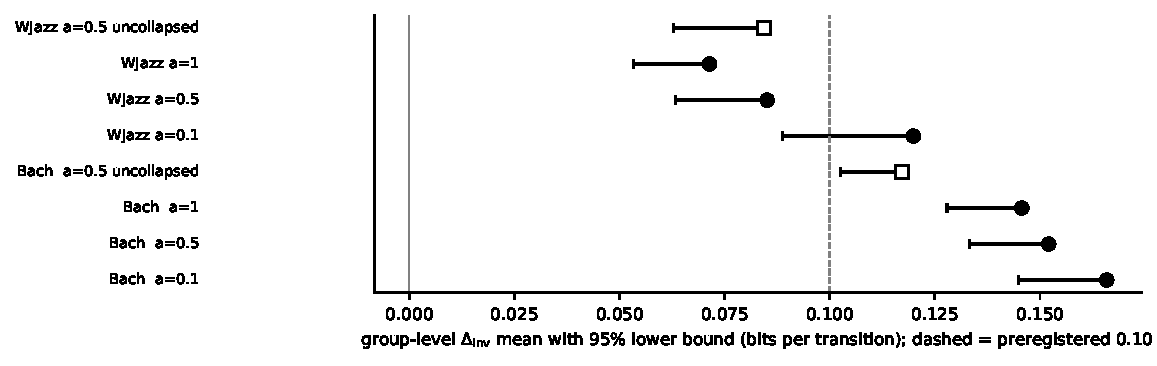
\includegraphics[width=\linewidth]{figs/fig4_lcb.pdf}\caption{Group-level $\Delta_{\mathrm{inv}}$ with 95\% lower bounds; dashed = preregistered 0.10 bits.}\end{figure}

\section{Edge drivers, named paths and cycle circulation}
\begin{table}[t]\centering\small\caption{Top directed edges by plug-in contribution to $\sigma$ (forward and reverse counts).}\label{tab:edges}
\begin{tabular}{lrrr}\toprule edge & forward & reverse & bits \\ \midrule
\multicolumn{4}{l}{\emph{Bach}} \\
V maj (major) -> I maj (major) & 1611 & 839 & 0.058 \\
II dim (minor) -> V maj (minor) & 193 & 4 & 0.040 \\
V maj (minor) -> I maj (minor) & 167 & 2 & 0.039 \\
IV maj (major) -> V maj (major) & 429 & 87 & 0.037 \\
IV min (minor) -> V maj (minor) & 214 & 10 & 0.035 \\
VII dim (major) -> I maj (major) & 390 & 76 & 0.035 \\
II maj (major) -> V maj (major) & 463 & 117 & 0.035 \\
bVII maj (minor) -> bIII maj (minor) & 579 & 206 & 0.033 \\
\multicolumn{4}{l}{\emph{WJazzD}} \\
II m7 (major) -> V 7 (major) & 1976 & 107 & 0.302 \\
V 7 (major) -> I maj7 (major) & 984 & 42 & 0.162 \\
VI 7 (major) -> II m7 (major) & 975 & 54 & 0.148 \\
III m7 (major) -> VI 7 (major) & 431 & 5 & 0.099 \\
V 7 (major) -> I 6 (major) & 438 & 24 & 0.066 \\
VI 7 (major) -> II 7 (major) & 279 & 3 & 0.064 \\
I 7 (major) -> IV maj7 (major) & 196 & 0 & 0.061 \\
II 7 (major) -> V 7 (major) & 332 & 12 & 0.057 \\
\bottomrule\end{tabular}\end{table}
\begin{table}[t]\centering\small
\caption{Fundamental-cycle decomposition of the stationary first-order fit (maximum symmetric-traffic spanning forest; $\sigma=\sum_C j_C A_C$ closes to machine precision: Bach $\sigma=0.864$, WJazzD $\sigma=2.156$; top-5 shares 28\% and 16\%). Terms are basis dependent; only the total is invariant.}\label{tab:cyc}
\begin{tabular}{llrrrr}\toprule corpus & fundamental cycle & $j_C$ & $A_C$ (bits) & $j_C A_C$ & share (\%) \\ \midrule
Bach & V:majm$\rightarrow$II:dimm$\rightarrow$I:minm$\rightarrow$V:majm & -0.00642 & -8.51 & 0.0546 & 6.3 \\
Bach & V:maj$\rightarrow$IV:maj$\rightarrow$I:maj$\rightarrow$V:maj & -0.01214 & -4.37 & 0.0530 & 6.1 \\
Bach & V:majm$\rightarrow$IV:minm$\rightarrow$bIII:majm$\rightarrow$I:minm$\rightarrow$V:majm & -0.00735 & -6.49 & 0.0477 & 5.5 \\
Bach & VII:dim$\rightarrow$IV:maj$\rightarrow$I:maj$\rightarrow$VII:dim & -0.00642 & -7.33 & 0.0471 & 5.5 \\
Bach & V:maj$\rightarrow$II:min$\rightarrow$I:maj$\rightarrow$V:maj & -0.01098 & -3.75 & 0.0412 & 4.8 \\
WJazzD & II:m7$\rightarrow$I:6$\rightarrow$V:7$\rightarrow$II:m7 & -0.00604 & -13.50 & 0.0815 & 3.8 \\
WJazzD & II:7$\rightarrow$I:6$\rightarrow$V:7$\rightarrow$II:7 & -0.00576 & -13.37 & 0.0770 & 3.6 \\
WJazzD & I:maj7$\rightarrow$VI:7$\rightarrow$II:m7$\rightarrow$V:7$\rightarrow$I:maj7 & 0.00400 & 16.20 & 0.0647 & 3.0 \\
WJazzD & I:7$\rightarrow$III:m7$\rightarrow$VI:7$\rightarrow$II:m7$\rightarrow$V:7$\rightarrow$I:7 & 0.00249 & 24.08 & 0.0600 & 2.8 \\
WJazzD & I:maj$\rightarrow$VI:7$\rightarrow$II:m7$\rightarrow$V:7$\rightarrow$I:maj & 0.00283 & 18.69 & 0.0530 & 2.5 \\
\bottomrule\end{tabular}\end{table}
\begin{table}[t]\centering\small
\caption{Named loops as contiguous four-state windows within works (collapsed events): forward and exactly reversed occurrences.}\label{tab:loops}
\begin{tabular}{llrrr}\toprule corpus & loop & forward & reverse & works with forward \\ \midrule
Bach & i$\rightarrow$iv$\rightarrow$V$\rightarrow$i & 20 & 0 & 19 \\
Bach & I$\rightarrow$IV$\rightarrow$V$\rightarrow$I & 115 & 4 & 94 \\
Bach & I$\rightarrow$ii$\rightarrow$V$\rightarrow$I & 165 & 8 & 109 \\
WJazzD & Imaj7$\rightarrow$ii7$\rightarrow$V7$\rightarrow$Imaj7 & 54 & 0 & 17 \\
WJazzD & Imaj7$\rightarrow$II7$\rightarrow$V7$\rightarrow$Imaj7 & 1 & 0 & 1 \\
WJazzD & Imaj7$\rightarrow$vi7$\rightarrow$ii7$\rightarrow$V7 & 0 & 0 & 0 \\
\bottomrule\end{tabular}\end{table}

\begin{figure}[t]\centering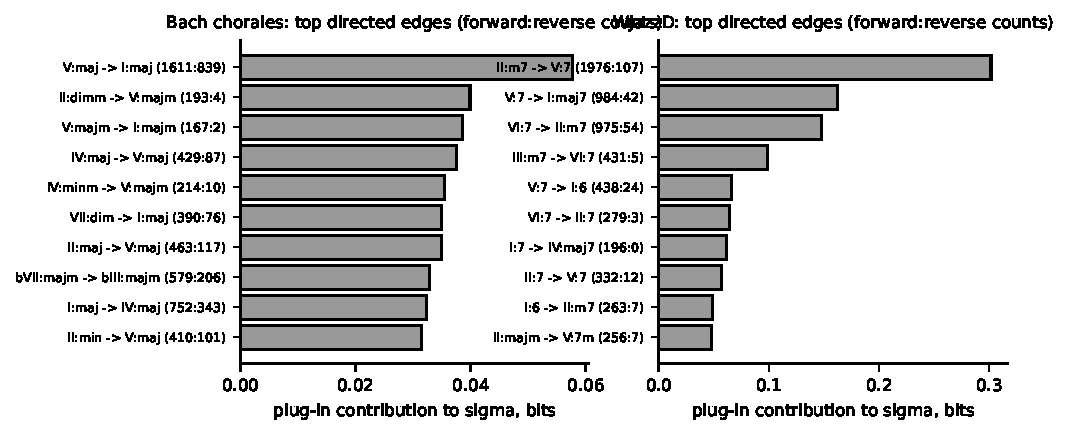
\includegraphics[width=\linewidth]{figs/fig5_edges.pdf}\caption{Top directed edges by contribution.}\end{figure}
\begin{figure}[t]\centering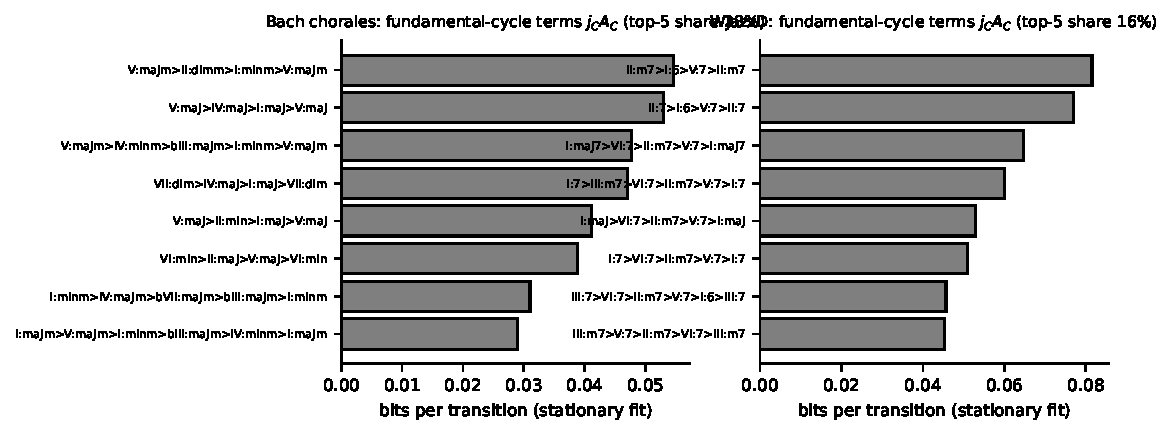
\includegraphics[width=\linewidth]{figs/fig6_cycles.pdf}\caption{Fundamental-cycle terms of the stationary fit.}\end{figure}
Depth-2 path asymmetry (plug-in) is 1.879 bits in Bach and 4.602 in WJazzD against 0.939 and 3.358 at the edge level; held-out path estimates are left for future work.

\section{Limitations and replication}
All quantities are descriptive of these two annotated corpora, their chord-type templates, key annotations (machine-estimated for Bach, annotated for WJazzD), event definitions and the fixed smoothing family. The inversion action is mode-conditioned pitch-class inversion; other $D_{12}$ actions are possible. Raw Bach and WJazzD magnitudes are not compared as a genre effect. Code and derived counts are released; every table regenerates from the JSON manifest.
\end{document}
